\documentclass{beamer}
%\documentclass[handout]{beamer}
\usetheme{neo}
\usepackage{tikz}
\usetikzlibrary{arrows,backgrounds,decorations.markings,shapes.misc}

% Gefunden auf: https://texample.net/tikz/examples/double-arrows/
\tikzstyle{vecArrow} = [thick, decoration={markings,mark=at position
    1 with {\arrow[semithick]{open triangle 60}}},
    double distance=1.4pt, shorten >= 5.5pt,
    preaction = {decorate},
    postaction = {draw,line width=1.4pt, white,shorten >= 4.5pt}]

% Siehe: https://tex.stackexchange.com/questions/123760/draw-crosses-in-tikz
\tikzset{cross/.style={cross out, draw=black, minimum size=2*(#1-\pgflinewidth), inner sep=0pt, outer sep=0pt, line width=2pt},
%default radius will be 1pt.
cross/.default={8pt}}

\usepackage[utf8]{inputenc} % UTF-8 Kodierung verwenden
\usepackage[ngerman]{babel} % Neue deutsche Sprache
\usepackage{textpos}
\usepackage[percent]{overpic}
\usepackage{soul}
\usepackage{pgfplots}
\usepackage{booktabs} % \midrule
\usepackage{makecell} % \makecell
\usepackage{smartdiagram}



\newcommand{\gerquot}[1]{\glqq#1\grqq}
\newcommand{\dashAndSpace}{\textendash \space}
\newcommand{\dashAndSpaceSeq}[1]{\dashAndSpace#1 \dashAndSpace}
\newcommand{\tikzScale}{0.75}
\newcommand{\massCharge}{$ m/z $ }
\newcommand{\xAxisUnit}{\massCharge}
\newcommand{\yAxisUnit}{$y$}
\newcommand{\yAxisHeight}{3}
\newcommand{\xAxisLength}{5}
\newcommand{\axisColorOffset}{0.15}



\title{De-Novo-Sequencing using Spectrum-Graphs, enabling Open Searches}
\author{Dominik Habermann}
\date{\today}

\institute{Ruhr Universität Bochum}



%%%%% %%%%% %%%%% %%%%% %%%%% %%%%% %%%%% %%%%%                %%%%% %%%%% %%%%% %%%%% %%%%% %%%%% %%%%% %%%%%
%%%%% %%%%% %%%%% %%%%% %%%%% %%%%% %%%%% %%%%% BEGIN document %%%%% %%%%% %%%%% %%%%% %%%%% %%%%% %%%%% %%%%%
%%%%% %%%%% %%%%% %%%%% %%%%% %%%%% %%%%% %%%%%                %%%%% %%%%% %%%%% %%%%% %%%%% %%%%% %%%%% %%%%%
\begin{document}
    \maketitle

    % * Praesentation fuer Bioinformatik Seminar *
    % - Dauer: 40 Min
    %
    % - Vortrag: 30 Min
    % - Diskussion / Fragen: 10 Min
    \begin{frame}{Gliederung}
    \tableofcontents
    \end{frame}

    \section{Hintergrund}
        \begin{frame}{Hintergrund}
        \onslide<1->{
            \begin{minipage}[t]{0.2\textwidth}
            \vspace*{0.5cm}
            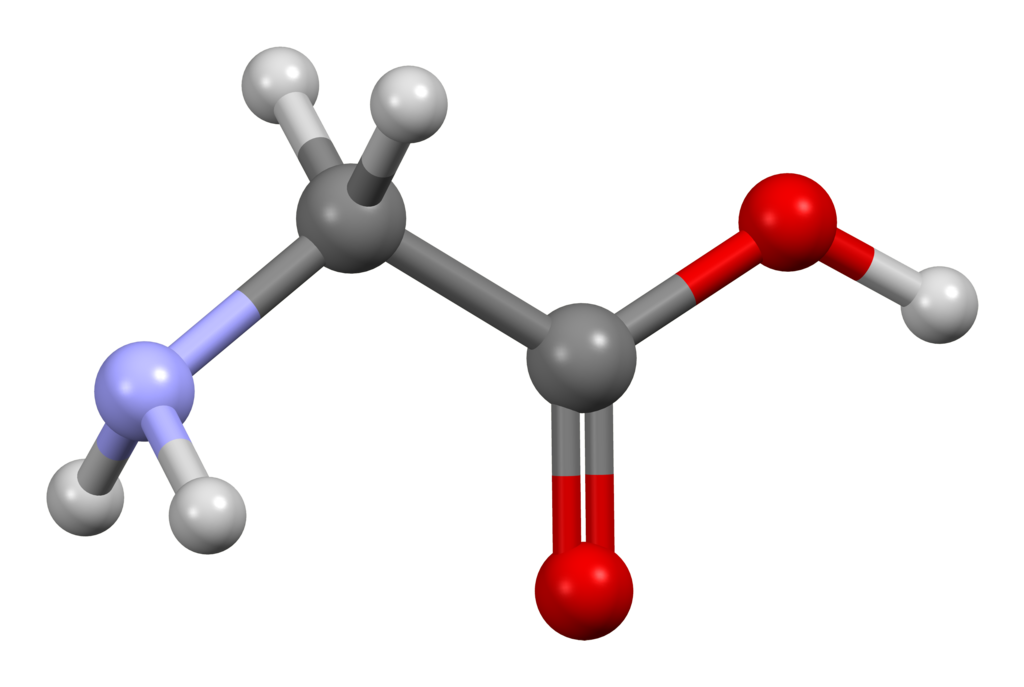
\includegraphics[scale=0.065]{./Presentation_Images/Glycine-neutral-Ipttt-conformer-3D-bs-17.png}
      \end{minipage}
            }%
            \onslide<1->{
            \begin{minipage}[t]{0.75\textwidth}
                \begin{itemize}
                  \item<1-> Peptide: Kette von Aminosäuren (AS)
                  \item<2-> 20 relevante AS
                  \item<3-> Reihenfolge von AS ist weitesgehend beliebig
                  \item<4-> $f(x)=20^x$\space\space\space$x:$ $Anzahl$ $an$ $AS$
                \end{itemize}
                % Bild von Grundaufbau einer AS
                \end{minipage}
            }
        \end{frame}
        \begin{frame}{Anzahl an Kombinationen}
         \onslide<1->{
         \begin{itemize}
          \item<1-> Bereits bei wenigen AS: Zu viele Kombinationen
         \end{itemize}

         }%
         \onslide<2->{
         \centering
         \begin{tikzpicture}[scale=0.75]
         \begin{axis} [axis lines=center,xlabel=$x$,
    ylabel={$f(x)=20^x$}]
            \addplot [domain=0:5, smooth, thick] { 20^x };
         \end{axis}
         \end{tikzpicture}
         }%
         \onslide<3->{
         \begin{itemize}
          \item<3-> Zum Vergleich: Proteine bis zu mehreren zehntausend AS
         \end{itemize}

         }%
        \end{frame}


        \begin{frame}{Biomedizinische Fragestellung}
        \onslide<1->{
         \begin{minipage}[t]{0.2\textwidth}
         \vspace*{0.5cm}
         
\includegraphics[scale=0.25]{./Presentation_Images/vecteezy_question-mark-with-3d-vector-icon-cartoon-minimal-style_16626300.png}
   \end{minipage}
         }%
        \onslide<1->{
        \begin{minipage}[t]{0.75\textwidth}
        \begin{itemize}
        \item<1-> Zuverlässige Bestimmung \emph{kurzkettiger} Peptide möglich?
        \item<2-> Biomedizinisch relevant:
        \begin{itemize}
         \item<3-> Katalogisierung von Proteinen
         \item<4-> Wechselwirkungen von Proteinen
         \item<5-> Analyse von Enzymen
        \end{itemize}
        \end{itemize}
        \end{minipage}
        }
        \end{frame}



    \section{AS Sequenzierung}
    \begin{frame}{AS Sequenzierung}
     \onslide<1->{
     \begin{itemize}
      \item<1-> AS Sequenzierung: Bestimmung der AS-Sequenz
      \item<2-> Hilfsmittel: Massenspektrometrie (MS)
      \item<3-> MS kann chemische Strukturen bestimmen
      \item<4-> Rückschluss auf die AS-Sequenz
     \end{itemize}
     }%
    \end{frame}

    \begin{frame}{Beispiel Massenspektrogramm}
    \onslide<1->{
        \begin{itemize}
         \item<1-> Ergebnisse einer MS: Massenspektrogramm
        \end{itemize}

    }%
    \onslide<2->{
    \centering
    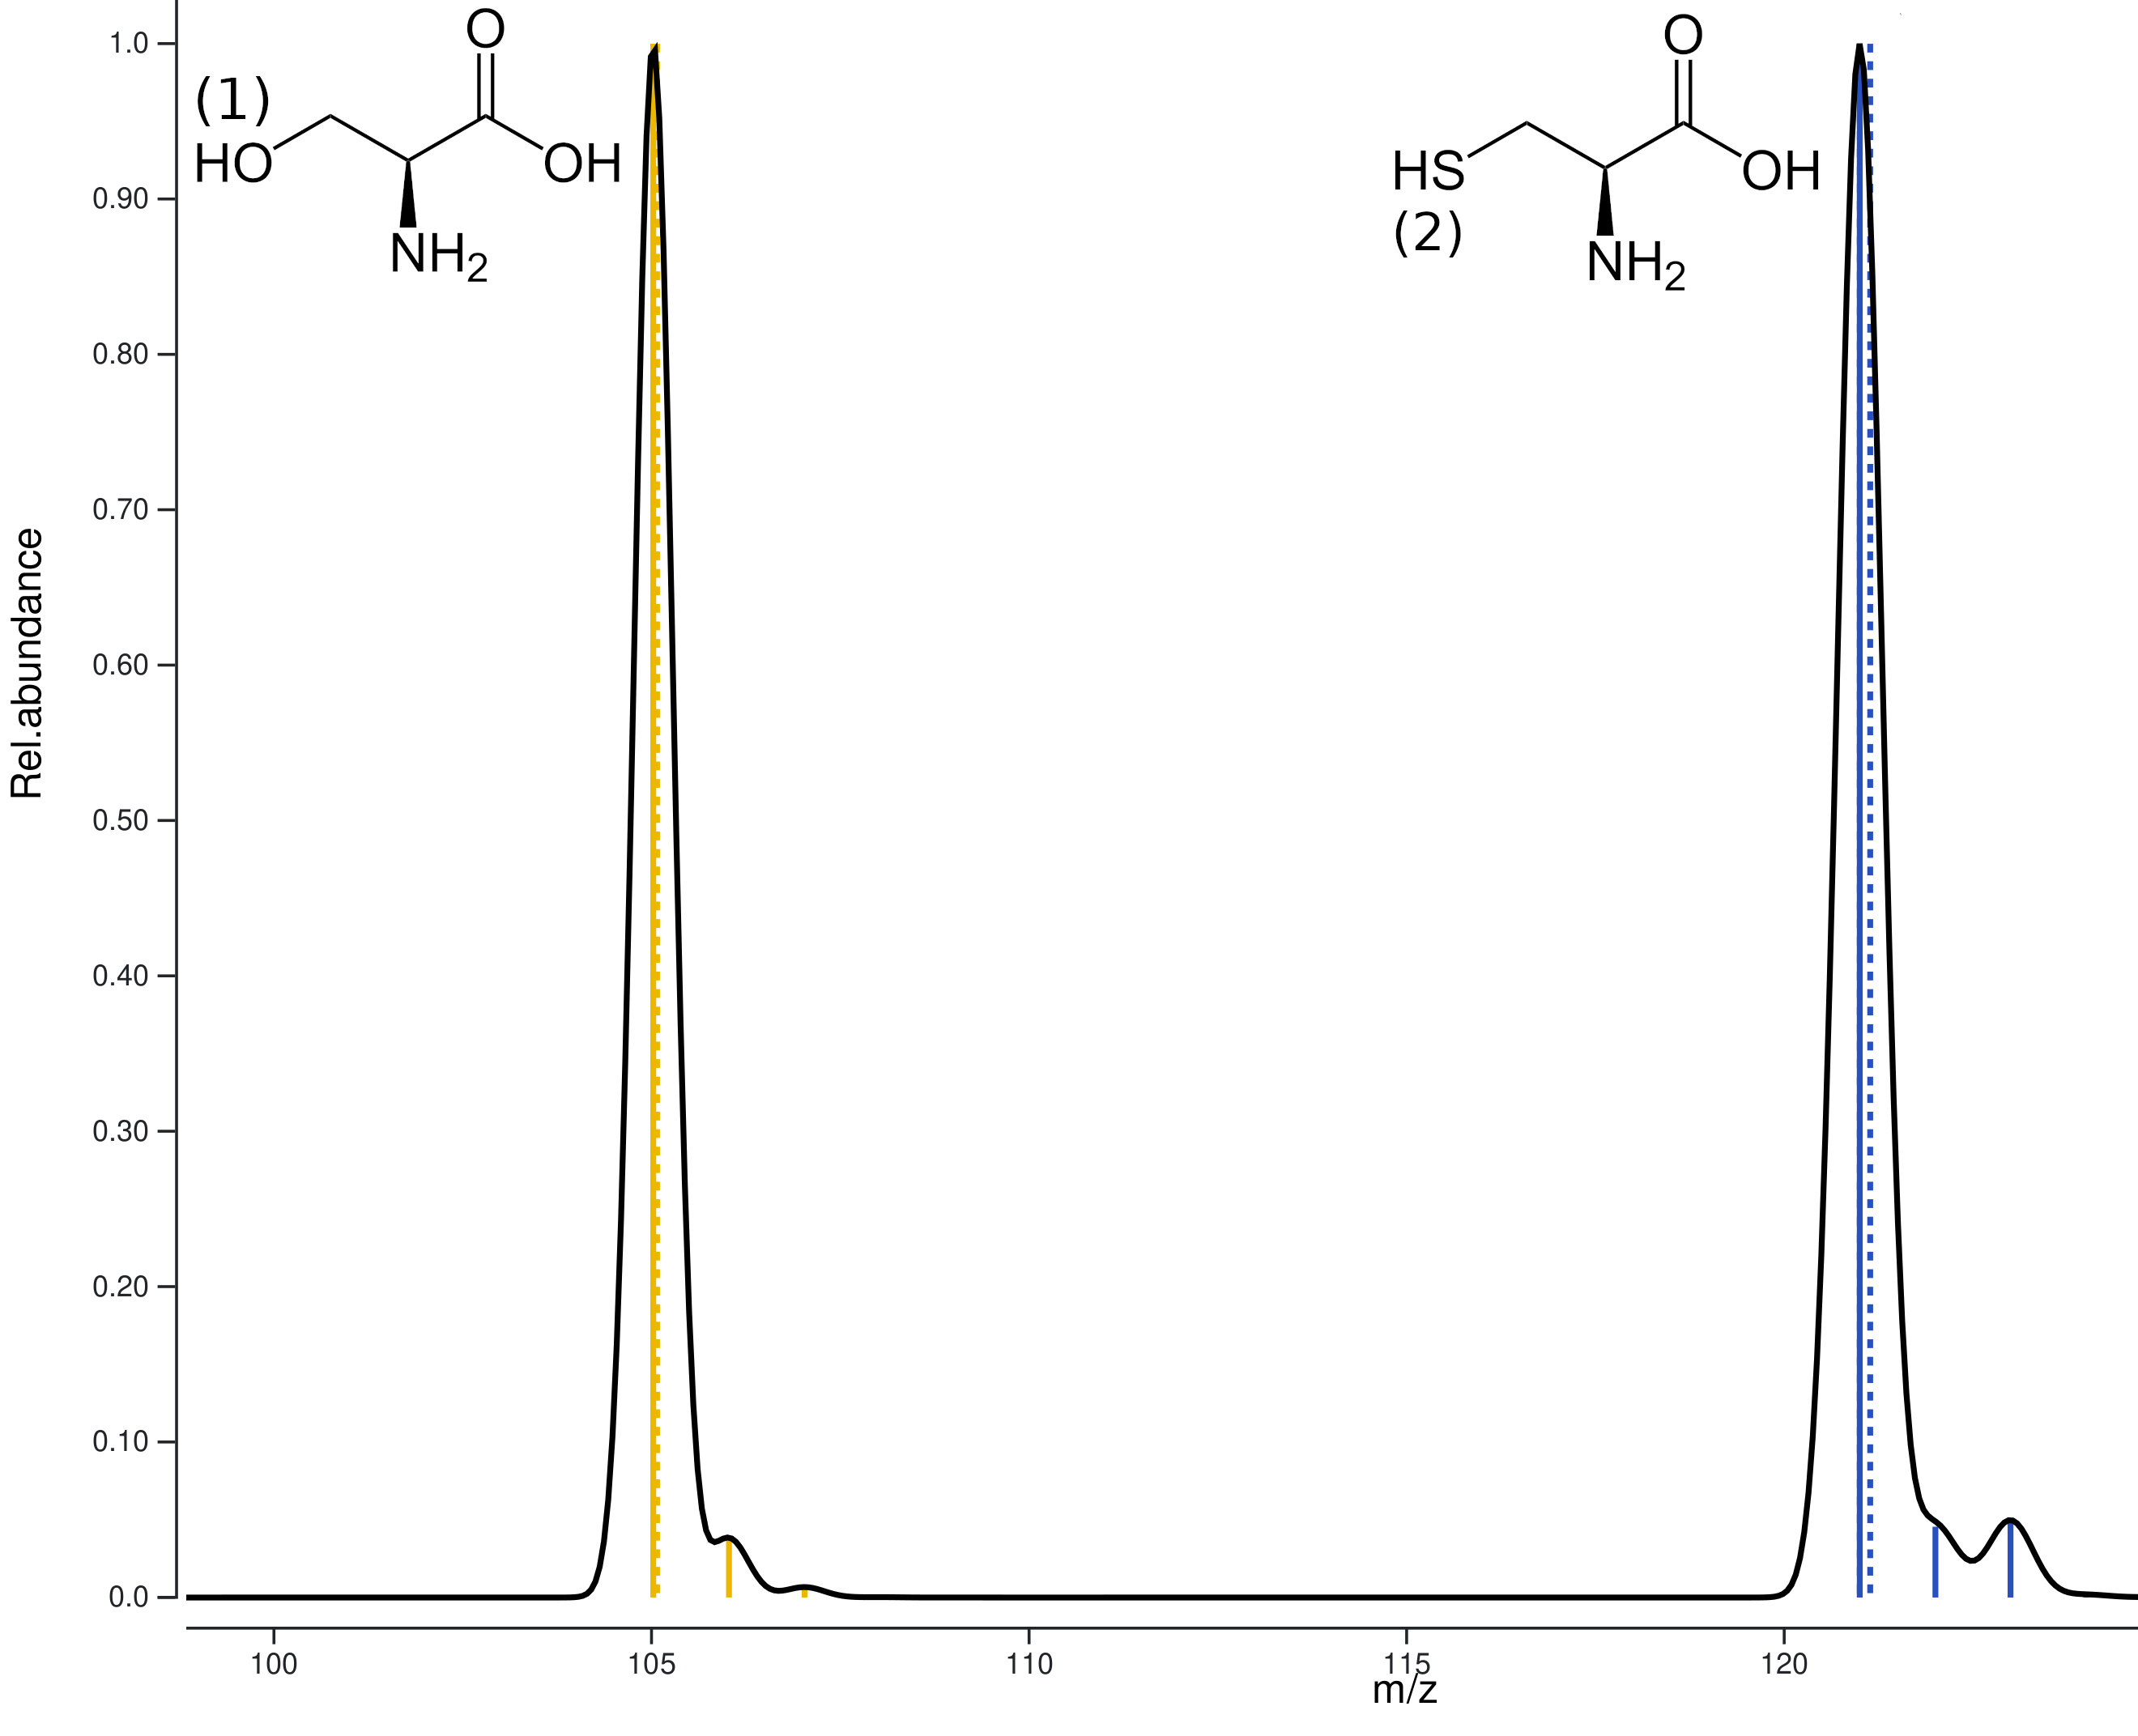
\includegraphics[scale=0.110]{./Resources/Simulated_Mass_Spectrum.png}
    }%
    \end{frame}



    \section{De-Novo-Sequenzierung}
    \begin{frame}{Sequenzierung und De-Novo-Sequenzierung}
     \onslide<1->{
     \begin{itemize}
      \item<1-> Beide Verfahren bestimmen die AS-Sequenz
     \end{itemize}
     \vspace*{0.5cm}
     }%

     \only<2>{
     \centering
     \begin{tabular}{c|c}
     AS Sequenzierung & De-Novo-Sequenzierung \\
     \midrule
     Datenbanken als \\Hilfsmittel & \\
      & \\
      & \\
     \end{tabular}
     }%

     \only<3>{
     \centering
     \begin{tabular}{c|c}
     AS Sequenzierung & De-Novo-Sequenzierung \\
     \midrule
     Datenbanken als \\Hilfsmittel & \\
      & \\
     \makecell{Identifizierung von \emph{bekannten}\\Sequenzen} & \\
     \end{tabular}
     }%

     \only<4>{
     \centering
     \begin{tabular}{c|c}
     AS Sequenzierung & De-Novo-Sequenzierung \\
     \midrule
     Datenbanken als \\Hilfsmittel & Ohne weitere Hilfsmittel\\
      & \\
     \makecell{Identifizierung von \emph{bekannten}\\Sequenzen} & \\
     \end{tabular}
     }%

     \only<5>{
     \centering
     \begin{tabular}{c|c}
     AS Sequenzierung & De-Novo-Sequenzierung \\
     \midrule
     Datenbanken als \\Hilfsmittel & Ohne weitere Hilfsmittel\\
      & \\
     \makecell{Identifizierung von \emph{bekannten}\\Sequenzen} & \makecell{Bestimmung \emph{unbekannter}\\Sequenzen}\\
     \end{tabular}
     }%

     \only<6>{
     \centering
     \begin{tabular}{c|c}
     AS Sequenzierung & De-Novo-Sequenzierung \\
     \midrule
     Datenbanken als \\Hilfsmittel & Ohne weitere Hilfsmittel\\
      & \\
     \makecell{Identifizierung von \emph{bekannten}\\Sequenzen} & \makecell{Bestimmung \emph{unbekannter}\\Sequenzen}\\
     \end{tabular}
     \vspace*{0.5cm}
     \begin{itemize}
      \item De novo: lat. \gerquot{Von neuem}
     \end{itemize}
     }%
     \end{frame}

    \begin{frame}{De-Novo-Sequenzierung (Sequenzierung ohne Datenbank)}
         \onslide<1->{
         \begin{minipage}[t]{0.2\textwidth}
         \smartdiagramset{back arrow disabled=true, module y sep =1,}
         \smartdiagram[flow diagram:vertical]{Edit,
  \LaTeX, Bib\TeX/ biber, make\-index, \LaTeX}
   \end{minipage}
         }%
         \onslide<1->
         {
         \begin{minipage}[t]{0.70\textwidth}
    \begin{itemize}
     \item<1-> Zusätzliche Informationen notwendig
     \item<2-> Verwendung einer 2. MS
     \item<3-> Sogenannte Tandem-Massenspektrometrie MS2
     % einfacher Graph, der den Ablauf zeigt
     \end{itemize}
     \end{minipage}
     }%
   \end{frame}

    \begin{frame}{De-Novo-Sequenzierung \dashAndSpace 1. MS}
    \begin{itemize}
      \item<1-> Ionen aus \massCharge Bereich auswählbar machen
      \item<2-> Quasi eine Filterung
      \item<3-> Ausgewählte Ionen werden für 2. MS verwendet
    \end{itemize}
    \end{frame}

    \begin{frame}{De-Novo-Sequenzierung \dashAndSpace 2. MS}
    \begin{itemize}
      \item<1-> Ionen aus 1. MS \gerquot{fragmentieren}:
      \begin{itemize}
       \item<2-> Energiezuführung
       \item<3-> Ionen zerfallen
       \item<4-> Ergebnis: \gerquot{Fragment-Ionen}
      \end{itemize}
      \item<2-> 2. MS wird auf Fragment-Ionen angewendet
    \end{itemize}
    \end{frame}

    \begin{frame}{De-Novo-Sequenzierung \dashAndSpace MS2}
    \begin{itemize}
      \item<1-> Höhere Genauigkeit durch Filterung nach 1. MS
      \item<2-> Bessere Selektivität beim 2. MS
      \item<3-> Fragment-Ionen zerfallen spezifisch
      \item<4-> $\rightarrow$ Rekonstruktion der ursprünglichen Ionen möglich
      \vspace*{0.5cm}
      \item<5-> MS2 Ergebnisse haben eine höhere Qualität
    \end{itemize}
    \end{frame}



    \section{pNovo+ Algorithmus}
    \begin{frame}{pNovo+ Algorithmus \dashAndSpace Übersicht}
    \begin{itemize}
    \item<1-> Algorithmus für die De-Novo-Sequenzierung
    \item<2-> Auswertung von MS2 Spektrogrammen
    \item<3-> Rekonstruktion der AS-Sequenz
    \item<4-> Spektrums-Graph
    \item<3-> Ziel: Qualität der Ergebnisse verbessern
    \end{itemize}
    \end{frame}

    \begin{frame}{pNovo+ Algorithmus \dashAndSpace Hauptansatz}
    \begin{itemize}
     \item<1-> \textbf{Zwei} MS2 Spektren verwenden
     \item<2-> Unterschiedliche Fragmentierungsmethoden
     \item<3-> Hintergrundrauschen aus den Daten entfernen
     \end{itemize}
    \end{frame}


    \begin{frame}{pNovo+ Algorithmus \dashAndSpace Datenaufbereitung}
    \newcommand{\minWidth}{4.5cm}
    \newcommand{\minHeight}{1.0cm}
    \newcommand{\minWidthOverview}{2.9cm}
    \newcommand{\minHeightOverview}{0.5cm}
    \newcommand{\xStartOverview}{3}
    \newcommand{\yStartOverview}{2}
    \only<1>{
         \centering
         \begin{tikzpicture}
        \node[rectangle,draw,text=black, fill=orange, minimum width=\minWidth, minimum height=\minHeight, align=center] (r1) at (0,0) {Hintergrundrauschen\\ verringern};
        %\node[rectangle,draw,text=black, fill=yellow, minimum width=\minWidth, minimum height=\minHeight, align=center] (r2) at (0,-1.75) {Entfernung falscher\\Peaks};
          %\node[rectangle,draw,text=black, fill=green, minimum width=\minWidth, minimum height=\minHeight, align=center] (r3) at (0,-3.5) {Entfernung irrelevanter\\ Peaks};
          %\node[rectangle,draw,text=black, fill=magenta, minimum width=\minWidth, minimum height=\minHeight, align=center] (r4) at (0,-5.25) {Zusammenfassen};
          %\draw[->, ultra thick] (r1) -- (r2);
          %\draw[->, ultra thick] (r2) -- (r3);
          %\draw[->, ultra thick] (r3) -- (r4);
         \end{tikzpicture}
         }%

         \only<2>{
              \centering
         \begin{tikzpicture}
        \node[rectangle,draw,text=black, fill=orange, minimum width=\minWidth, minimum height=\minHeight, align=center] (r1) at (0,0) {Hintergrundrauschen\\ verringern};
        \node[rectangle,draw,text=black, fill=yellow, minimum width=\minWidth, minimum height=\minHeight, align=center] (r2) at (0,-1.75) {Entfernung falscher\\Peaks};
          %\node[rectangle,draw,text=black, fill=green, minimum width=\minWidth, minimum height=\minHeight, align=center] (r3) at (0,-3.5) {Entfernung irrelevanter\\ Peaks};
          %\node[rectangle,draw,text=black, fill=magenta, minimum width=\minWidth, minimum height=\minHeight, align=center] (r4) at (0,-5.25) {Zusammenfassen};
          \draw[->, ultra thick] (r1) -- (r2);
          %\draw[->, ultra thick] (r2) -- (r3);
          %\draw[->, ultra thick] (r3) -- (r4);
         \end{tikzpicture}
         }%

         \only<3>{
              \centering
         \begin{tikzpicture}
        \node[rectangle,draw,text=black, fill=orange, minimum width=\minWidth, minimum height=\minHeight, align=center] (r1) at (0,0) {Hintergrundrauschen\\ verringern};
        \node[rectangle,draw,text=black, fill=yellow, minimum width=\minWidth, minimum height=\minHeight, align=center] (r2) at (0,-1.75) {Entfernung falscher\\Peaks};
          \node[rectangle,draw,text=black, fill=green, minimum width=\minWidth, minimum height=\minHeight, align=center] (r3) at (0,-3.5) {Entfernung irrelevanter\\ Peaks};
          %\node[rectangle,draw,text=black, fill=magenta, minimum width=\minWidth, minimum height=\minHeight, align=center] (r4) at (0,-5.25) {Zusammenfassen};
          \draw[->, ultra thick] (r1) -- (r2);
          \draw[->, ultra thick] (r2) -- (r3);
          %\draw[->, ultra thick] (r3) -- (r4);
         \end{tikzpicture}
         }%

         \only<4>{
              \centering
         \begin{tikzpicture}
        \node[rectangle,draw,text=black, fill=orange, minimum width=\minWidth, minimum height=\minHeight, align=center] (r1) at (0,0) {Hintergrundrauschen\\ verringern};
        \node[rectangle,draw,text=black, fill=yellow, minimum width=\minWidth, minimum height=\minHeight, align=center] (r2) at (0,-1.75) {Entfernung falscher\\Peaks};
          \node[rectangle,draw,text=black, fill=green, minimum width=\minWidth, minimum height=\minHeight, align=center] (r3) at (0,-3.5) {Entfernung irrelevanter\\ Peaks};
          \node[rectangle,draw,text=black, fill=magenta, minimum width=\minWidth, minimum height=\minHeight, align=center] (r4) at (0,-5.25) {Zusammenfassen};
          \draw[->, ultra thick] (r1) -- (r2);
          \draw[->, ultra thick] (r2) -- (r3);
          \draw[->, ultra thick] (r3) -- (r4);
         \end{tikzpicture}
         }%

         \only<5>{
              \centering
         \begin{tikzpicture}[font=\scriptsize]
        \node[rectangle,draw,text=black, fill=orange, minimum width=\minWidthOverview, minimum height=\minHeightOverview, align=center] (r1) at (\xStartOverview,\yStartOverview) {Hintergrundrauschen};
        \node[rectangle,draw,text=black, fill=yellow, minimum width=\minWidthOverview, minimum height=\minHeightOverview, align=center] (r2) at (\xStartOverview,\yStartOverview-1) {Falsche Peaks};
          \node[rectangle,draw,text=black, fill=green, minimum width=\minWidthOverview, minimum height=\minHeightOverview, align=center] (r3) at (\xStartOverview,\yStartOverview-2) {Irrelevante Peaks};
          \node[rectangle,draw,text=black, fill=magenta, minimum width=\minWidthOverview, minimum height=\minHeightOverview, align=center] (r4) at (\xStartOverview,\yStartOverview-3) {Zusammenfassen};
          \draw[->, ultra thick] (r1) -- (r2);
          \draw[->, ultra thick] (r2) -- (r3);
          \draw[->, ultra thick] (r3) -- (r4);
         \end{tikzpicture}
         }%
    \end{frame}

    \begin{frame}{pNovo+ Algorithmus \dashAndSpace Datenaufbereitung}
    \begin{itemize}
    \item<1-> Hintergrundrauschen reduzieren
    \item<2-> Anwendung $ln()$
    \end{itemize}
\onslide<3-> {
   \begin{minipage}[t]{0.45\textwidth}
      \centering
      \begin{tikzpicture}[scale=\tikzScale, baseline=(current bounding box.center)]
         \draw [<->,thick] (0,\yAxisHeight) node (yaxis) [above] {\yAxisUnit}
         |- (\xAxisLength,0) node (xaxis) [right] {\xAxisUnit};
\draw[thick] (0.2, 0.0) -- (0.2, 2.3);
\draw[thick] (0.382, 0.0) -- (0.382, 1.7);
\draw[thick] (0.476, 0.0) -- (0.476, 2.7);
\draw[thick] (0.456, 0.0) -- (0.456, 1.8);
\draw[thick] (0.6859999999999999, 0.0) -- (0.6859999999999999, 2.7);
\draw[thick] (0.6839999999999999, 0.0) -- (0.6839999999999999, 1.8);
\draw[thick] (0.752, 0.0) -- (0.752, 1.1);
\draw[thick] (0.8200000000000001, 0.0) -- (0.8200000000000001, 2.2);
\draw[thick] (1.076, 0.0) -- (1.076, 1.5);
\draw[thick] (1.16, 0.0) -- (1.16, 1.9);
\draw[thick] (1.2120000000000002, 0.0) -- (1.2120000000000002, 2.0);
\draw[thick] (1.28, 0.0) -- (1.28, 1.9);
\draw[thick] (1.452, 0.0) -- (1.452, 1.3);
\draw[thick] (1.426, 0.0) -- (1.426, 1.9);
\draw[thick] (1.548, 0.0) -- (1.548, 1.9);
\draw[thick] (1.6740000000000002, 0.0) -- (1.6740000000000002, 1.5);
\draw[thick] (1.788, 0.0) -- (1.788, 2.5);
\draw[thick] (1.856, 0.0) -- (1.856, 2.3);
\draw[thick] (2.036, 0.0) -- (2.036, 1.7);
\draw[thick] (2.142, 0.0) -- (2.142, 1.6);
\draw[thick] (2.2520000000000002, 0.0) -- (2.2520000000000002, 2.0);
\draw[thick] (2.386, 0.0) -- (2.386, 1.6);
\draw[thick] (2.488, 0.0) -- (2.488, 2.9);
\draw[thick] (2.4739999999999998, 0.0) -- (2.4739999999999998, 2.7);
\draw[thick] (2.504, 0.0) -- (2.504, 2.0);
\draw[thick] (2.682, 0.0) -- (2.682, 2.0);
\draw[thick] (2.702, 0.0) -- (2.702, 2.5);
\draw[thick] (2.9259999999999997, 0.0) -- (2.9259999999999997, 2.8);
\draw[thick] (3.024, 0.0) -- (3.024, 2.4);
\draw[thick] (3.096, 0.0) -- (3.096, 1.8);
\draw[thick] (3.244, 0.0) -- (3.244, 2.6);
\draw[thick] (3.362, 0.0) -- (3.362, 1.9);
\draw[thick] (3.46, 0.0) -- (3.46, 2.3);
\draw[thick] (3.516, 0.0) -- (3.516, 1.1);
\draw[thick] (3.584, 0.0) -- (3.584, 1.8);
\draw[thick] (3.652, 0.0) -- (3.652, 2.0);
\draw[thick] (3.838, 0.0) -- (3.838, 1.5);
\draw[thick] (3.8819999999999997, 0.0) -- (3.8819999999999997, 2.6);
\draw[thick] (4.088, 0.0) -- (4.088, 2.6);
\draw[thick] (4.046, 0.0) -- (4.046, 1.1);
\draw[thick] (4.167999999999999, 0.0) -- (4.167999999999999, 2.0);
\draw[thick] (4.266, 0.0) -- (4.266, 2.4);
\draw[thick] (4.38, 0.0) -- (4.38, 1.1);
\draw[thick] (4.456, 0.0) -- (4.456, 2.2);
\draw[thick] (4.644, 0.0) -- (4.644, 2.6);
\draw[thick] (4.675999999999999, 0.0) -- (4.675999999999999, 2.5);
\draw[thick] (4.898000000000001, 0.0) -- (4.898000000000001, 1.2);
   \end{tikzpicture}%
   \end{minipage}%
   }
   \onslide<4->{
   \textbf{$\rightarrow$}
   }%
   \onslide<5->{
   \begin{minipage}[t]{0.45\textwidth}
      \centering
      \begin{tikzpicture}[scale=\tikzScale, baseline=(current bounding box.center)]
      \draw [<->,thick] (0,\yAxisHeight) node (yaxis) [above] {\yAxisUnit}
      |- (\xAxisLength,0) node (xaxis) [right] {\xAxisUnit};
\draw[thick] (0.2, 0.0) -- (0.2, {ln(2.3)});
\draw[thick] (0.382, 0.0) -- (0.382, {ln(1.7)});
\draw[thick] (0.476, 0.0) -- (0.476, {ln(2.7)});
\draw[thick] (0.456, 0.0) -- (0.456, {ln(1.8)});
\draw[thick] (0.6859999999999999, 0.0) -- (0.6859999999999999, {ln(2.7)});
\draw[thick] (0.6839999999999999, 0.0) -- (0.6839999999999999, {ln(1.8)});
\draw[thick] (0.752, 0.0) -- (0.752, {ln(1.1)});
\draw[thick] (0.8200000000000001, 0.0) -- (0.8200000000000001, {ln(2.2)});
\draw[thick] (1.076, 0.0) -- (1.076, {ln(1.5)});
\draw[thick] (1.16, 0.0) -- (1.16, {ln(1.9)});
\draw[thick] (1.2120000000000002, 0.0) -- (1.2120000000000002, {ln(2.0)});
\draw[thick] (1.28, 0.0) -- (1.28, {ln(1.9)});
\draw[thick] (1.452, 0.0) -- (1.452, {ln(1.3)});
\draw[thick] (1.426, 0.0) -- (1.426, {ln(1.9)});
\draw[thick] (1.548, 0.0) -- (1.548, {ln(1.9)});
\draw[thick] (1.6740000000000002, 0.0) -- (1.6740000000000002, {ln(1.5)});
\draw[thick] (1.788, 0.0) -- (1.788, {ln(2.5)});
\draw[thick] (1.856, 0.0) -- (1.856, {ln(2.3)});
\draw[thick] (2.036, 0.0) -- (2.036, {ln(1.7)});
\draw[thick] (2.142, 0.0) -- (2.142, {ln(1.6)});
\draw[thick] (2.2520000000000002, 0.0) -- (2.2520000000000002, {ln(2.0)});
\draw[thick] (2.386, 0.0) -- (2.386, {ln(1.6)});
\draw[thick] (2.488, 0.0) -- (2.488, {ln(2.9)});
\draw[thick] (2.4739999999999998, 0.0) -- (2.4739999999999998, {ln(2.7)});
\draw[thick] (2.504, 0.0) -- (2.504, {ln(2.0)});
\draw[thick] (2.682, 0.0) -- (2.682, {ln(2.0)});
\draw[thick] (2.702, 0.0) -- (2.702, {ln(2.5)});
\draw[thick] (2.9259999999999997, 0.0) -- (2.9259999999999997, {ln(2.8)});
\draw[thick] (3.024, 0.0) -- (3.024, {ln(2.4)});
\draw[thick] (3.096, 0.0) -- (3.096, {ln(1.8)});
\draw[thick] (3.244, 0.0) -- (3.244, {ln(2.6)});
\draw[thick] (3.362, 0.0) -- (3.362, {ln(1.9)});
\draw[thick] (3.46, 0.0) -- (3.46, {ln(2.3)});
\draw[thick] (3.516, 0.0) -- (3.516, {ln(1.1)});
\draw[thick] (3.584, 0.0) -- (3.584, {ln(1.8)});
\draw[thick] (3.652, 0.0) -- (3.652, {ln(2.0)});
\draw[thick] (3.838, 0.0) -- (3.838, {ln(1.5)});
\draw[thick] (3.8819999999999997, 0.0) -- (3.8819999999999997, {ln(2.6)});
\draw[thick] (4.088, 0.0) -- (4.088, {ln(2.6)});
\draw[thick] (4.046, 0.0) -- (4.046, {ln(1.1)});
\draw[thick] (4.167999999999999, 0.0) -- (4.167999999999999, {ln(2.0)});
\draw[thick] (4.266, 0.0) -- (4.266, {ln(2.4)});
\draw[thick] (4.38, 0.0) -- (4.38, {ln(1.1)});
\draw[thick] (4.456, 0.0) -- (4.456, {ln(2.2)});
\draw[thick] (4.644, 0.0) -- (4.644, {ln(2.6)});
\draw[thick] (4.675999999999999, 0.0) -- (4.675999999999999, {ln(2.5)});
\draw[thick] (4.898000000000001, 0.0) -- (4.898000000000001, {ln(1.2)});
      \end{tikzpicture}
      \end{minipage}
      }%
    \end{frame}

    \begin{frame}{pNovo+ Algorithmus \dashAndSpace Datenaufbereitung}
    \begin{itemize}
     \item<1-> Entfernen von falschen Peaks
     \item<2->
    \end{itemize}
    \onslide<3-> {
       \begin{minipage}[t]{.45\linewidth}
      \centering
      \begin{tikzpicture}[scale=\tikzScale, baseline=(current bounding box.center)]
         \draw [<->,thick] (0,\yAxisHeight) node (yaxis) [above] {\yAxisUnit}
         |- (\xAxisLength,0) node (xaxis) [right] {\xAxisUnit};
\draw[thick] (0.2, 0.0) -- (0.2, {ln(2.3)});
\draw[color=blue!85!,opacity=.55,thick] (0.382, 0.0) -- (0.382, {ln(1.7)});
\draw[color=blue!85!,opacity=.55,thick] (0.476, 0.0) -- (0.476, {ln(2.7)});
\draw[color=magenta,thick] (0.456, 0.0) -- (0.456, {ln(1.8)});
\draw[color=blue!85!,opacity=.55,thick] (0.6859999999999999, 0.0) -- (0.6859999999999999, {ln(2.7)});
\draw[color=blue!85!,opacity=.55,thick] (0.6839999999999999, 0.0) -- (0.6839999999999999, {ln(1.8)});
\draw[thick] (0.752, 0.0) -- (0.752, {ln(1.1)});
\draw[thick] (0.8200000000000001, 0.0) -- (0.8200000000000001, {ln(2.2)});
\draw[thick] (1.076, 0.0) -- (1.076, {ln(1.5)});
\draw[thick] (1.16, 0.0) -- (1.16, {ln(1.9)});
\draw[thick] (1.2120000000000002, 0.0) -- (1.2120000000000002, {ln(2.0)});
\draw[thick] (1.28, 0.0) -- (1.28, {ln(1.9)});
\draw[color=blue!85!,opacity=.55,thick] (1.452, 0.0) -- (1.452, {ln(1.3)});
\draw[color=blue!85!,opacity=.55,thick] (1.426, 0.0) -- (1.426, {ln(1.9)});
\draw[color=magenta,thick] (1.548, 0.0) -- (1.548, {ln(1.9)});
\draw[color=blue!85!,opacity=.55,thick] (1.6740000000000002, 0.0) -- (1.6740000000000002, {ln(1.5)});
\draw[color=blue!85!,opacity=.55,thick] (1.788, 0.0) -- (1.788, {ln(2.5)});
\draw[thick] (1.856, 0.0) -- (1.856, {ln(2.3)});
\draw[thick] (2.036, 0.0) -- (2.036, {ln(1.7)});
\draw[thick] (2.142, 0.0) -- (2.142, {ln(1.6)});
\draw[thick] (2.2520000000000002, 0.0) -- (2.2520000000000002, {ln(2.0)});
\draw[thick] (2.386, 0.0) -- (2.386, {ln(1.6)});
\draw[color=blue!85!,opacity=.55,thick] (2.488, 0.0) -- (2.488, {ln(2.9)});
\draw[thick] (2.4739999999999998, 0.0) -- (2.4739999999999998, {ln(2.7)});
\draw[color=blue!85!,opacity=.55,thick] (2.504, 0.0) -- (2.504, {ln(2.0)});
\draw[color=magenta,thick] (2.682, 0.0) -- (2.682, {ln(2.0)});
\draw[color=blue!85!,opacity=.55,thick] (2.702, 0.0) -- (2.702, {ln(2.5)});
\draw[thick] (2.9259999999999997, 0.0) -- (2.9259999999999997, {ln(2.8)});
\draw[thick] (3.024, 0.0) -- (3.024, {ln(2.4)});
\draw[thick] (3.096, 0.0) -- (3.096, {ln(1.8)});
\draw[thick] (3.244, 0.0) -- (3.244, {ln(2.6)});
\draw[thick] (3.362, 0.0) -- (3.362, {ln(1.9)});
\draw[color=blue!85!,opacity=.55,thick] (3.46, 0.0) -- (3.46, {ln(2.3)});
\draw[color=blue!85!,opacity=.55,thick] (3.516, 0.0) -- (3.516, {ln(1.1)});
\draw[color=blue!85!,opacity=.55,thick] (3.584, 0.0) -- (3.584, {ln(1.8)});
\draw[color=magenta,thick] (3.652, 0.0) -- (3.652, {ln(2.0)});
\draw[color=blue!85!,opacity=.55,thick] (3.838, 0.0) -- (3.838, {ln(1.5)});
\draw[color=blue!85!,opacity=.55,thick] (3.8819999999999997, 0.0) -- (3.8819999999999997, {ln(2.6)});
\draw[thick] (4.088, 0.0) -- (4.088, {ln(2.6)});
\draw[thick] (4.046, 0.0) -- (4.046, {ln(1.1)});
\draw[thick] (4.167999999999999, 0.0) -- (4.167999999999999, {ln(2.0)});
\draw[thick] (4.266, 0.0) -- (4.266, {ln(2.4)});
\draw[color=blue!85!,opacity=.55,thick] (4.38, 0.0) -- (4.38, {ln(1.1)});
\draw[color=blue!85!,opacity=.55,thick] (4.456, 0.0) -- (4.456, {ln(2.2)});
\draw[color=magenta,thick] (4.644, 0.0) -- (4.644, {ln(2.6)});
\draw[color=blue!85!,opacity=.55,thick] (4.675999999999999, 0.0) -- (4.675999999999999, {ln(2.5)});
\draw[color=blue!85!,opacity=.55,thick] (4.898000000000001, 0.0) -- (4.898000000000001, {ln(1.2)});
   \end{tikzpicture}%
   \end{minipage}%
   }%
   \onslide<4-> {
   \textbf{$\rightarrow$}
   }%
   \onslide<5-> {
   \begin{minipage}[t]{.45\linewidth}
      \centering
      \begin{tikzpicture}[scale=\tikzScale, baseline=(current bounding box.center)]
      \draw [<->,thick] (0,\yAxisHeight) node (yaxis) [above] {\yAxisUnit}
      |- (\xAxisLength,0) node (xaxis) [right] {\xAxisUnit};
\draw[color=blue!85!,opacity=.55,thick] (0.382, 0.0) -- (0.382, {ln(1.7)});
\draw[color=blue!85!,opacity=.55,thick] (0.476, 0.0) -- (0.476, {ln(2.7)});
\draw[color=magenta,thick] (0.456, 0.0) -- (0.456, {ln(1.8)});
\draw[color=blue!85!,opacity=.55,thick] (0.6859999999999999, 0.0) -- (0.6859999999999999, {ln(2.7)});
\draw[color=blue!85!,opacity=.55,thick] (0.6839999999999999, 0.0) -- (0.6839999999999999, {ln(1.8)});
\draw[color=blue!85!,opacity=.55,thick] (1.452, 0.0) -- (1.452, {ln(1.3)});
\draw[color=blue!85!,opacity=.55,thick] (1.426, 0.0) -- (1.426, {ln(1.9)});
\draw[color=magenta,thick] (1.548, 0.0) -- (1.548, {ln(1.9)});
\draw[color=blue!85!,opacity=.55,thick] (1.6740000000000002, 0.0) -- (1.6740000000000002, {ln(1.5)});
\draw[color=blue!85!,opacity=.55,thick] (1.788, 0.0) -- (1.788, {ln(2.5)});
\draw[color=blue!85!,opacity=.55,thick] (2.488, 0.0) -- (2.488, {ln(2.9)});
\draw[color=blue!85!,opacity=.55,thick] (2.504, 0.0) -- (2.504, {ln(2.0)});
\draw[color=magenta,thick] (2.682, 0.0) -- (2.682, {ln(2.0)});
\draw[color=blue!85!,opacity=.55,thick] (2.702, 0.0) -- (2.702, {ln(2.5)});
\draw[color=blue!85!,opacity=.55,thick] (3.46, 0.0) -- (3.46, {ln(2.3)});
\draw[color=blue!85!,opacity=.55,thick] (3.516, 0.0) -- (3.516, {ln(1.1)});
\draw[color=blue!85!,opacity=.55,thick] (3.584, 0.0) -- (3.584, {ln(1.8)});
\draw[color=magenta,thick] (3.652, 0.0) -- (3.652, {ln(2.0)});
\draw[color=blue!85!,opacity=.55,thick] (3.838, 0.0) -- (3.838, {ln(1.5)});
\draw[color=blue!85!,opacity=.55,thick] (3.8819999999999997, 0.0) -- (3.8819999999999997, {ln(2.6)});
\draw[color=blue!85!,opacity=.55,thick] (4.38, 0.0) -- (4.38, {ln(1.1)});
\draw[color=blue!85!,opacity=.55,thick] (4.456, 0.0) -- (4.456, {ln(2.2)});
\draw[color=magenta,thick] (4.644, 0.0) -- (4.644, {ln(2.6)});
\draw[color=blue!85!,opacity=.55,thick] (4.675999999999999, 0.0) -- (4.675999999999999, {ln(2.5)});
\draw[color=blue!85!,opacity=.55,thick] (4.898000000000001, 0.0) -- (4.898000000000001, {ln(1.2)});
      \end{tikzpicture}
      \end{minipage}
}%
    \end{frame}


    \begin{frame}{pNovo+ Algorithmus \dashAndSpace Datenaufbereitung}
     \begin{itemize}
      \item<1-> Entfernen von Peaks aus einem irrelevanten Bereich
     \end{itemize}
     \onslide<2-> {
        \begin{minipage}[t]{.45\linewidth}
      \centering
      \begin{tikzpicture}[scale=\tikzScale, baseline=(current bounding box.center)]
         \draw [<->,thick] (0,\yAxisHeight) node (yaxis) [above] {\yAxisUnit}
         |- (\xAxisLength,0) node (xaxis) [right] {\xAxisUnit};
\draw[thick] (0.382, 0.0) -- (0.382, {ln(1.7)});
\draw[thick] (0.476, 0.0) -- (0.476, {ln(2.7)});
\draw[thick] (0.456, 0.0) -- (0.456, {ln(1.8)});
\draw[thick] (0.6859999999999999, 0.0) -- (0.6859999999999999, {ln(2.7)});
\draw[thick] (0.6839999999999999, 0.0) -- (0.6839999999999999, {ln(1.8)});
\draw[thick] (1.452, 0.0) -- (1.452, {ln(1.3)});
\draw[thick] (1.426, 0.0) -- (1.426, {ln(1.9)});
\draw[thick] (1.548, 0.0) -- (1.548, {ln(1.9)});
\draw[thick] (1.6740000000000002, 0.0) -- (1.6740000000000002, {ln(1.5)});
\draw[thick] (1.788, 0.0) -- (1.788, {ln(2.5)});
\draw[thick] (2.488, 0.0) -- (2.488, {ln(2.9)});
\draw[thick] (2.504, 0.0) -- (2.504, {ln(2.0)});
\draw[thick] (2.682, 0.0) -- (2.682, {ln(2.0)});
\draw[thick] (2.702, 0.0) -- (2.702, {ln(2.5)});
\draw[thick] (3.46, 0.0) -- (3.46, {ln(2.3)});
\draw[thick] (3.516, 0.0) -- (3.516, {ln(1.1)});
\draw[thick] (3.584, 0.0) -- (3.584, {ln(1.8)});
\draw[thick] (3.652, 0.0) -- (3.652, {ln(2.0)});
\draw[thick] (3.838, 0.0) -- (3.838, {ln(1.5)});
\draw[thick] (3.8819999999999997, 0.0) -- (3.8819999999999997, {ln(2.6)});
\draw[thick] (4.38, 0.0) -- (4.38, {ln(1.1)});
\draw[thick] (4.456, 0.0) -- (4.456, {ln(2.2)});
\draw[thick] (4.644, 0.0) -- (4.644, {ln(2.6)});
\draw[thick] (4.675999999999999, 0.0) -- (4.675999999999999, {ln(2.5)});
\draw[thick] (4.898000000000001, 0.0) -- (4.898000000000001, {ln(1.2)});

\fill[red!25!,opacity=.25] (0,0) rectangle (1,\yAxisHeight-\axisColorOffset);
         \fill[red!25!,opacity=.25] (\xAxisLength-1,0) rectangle (\xAxisLength-\axisColorOffset,\yAxisHeight-\axisColorOffset);
         \fill[green!25!,opacity=.25] (1,0) rectangle (\xAxisLength-1,\yAxisHeight-\axisColorOffset);
   \end{tikzpicture}%
   \end{minipage}%
     }%
     \onslide<3-> {
     \textbf{$\rightarrow$}
     }%
     \onslide<4->{
        \begin{minipage}[t]{.45\linewidth}
      \centering
      \begin{tikzpicture}[scale=\tikzScale, baseline=(current bounding box.center)]
         \draw [<->,thick] (0,\yAxisHeight) node (yaxis) [above] {\yAxisUnit}
         |- (\xAxisLength,0) node (xaxis) [right] {\xAxisUnit};
%\draw[thick] (0.382, 0.0) -- (0.382, {ln(1.7)});
%\draw[thick] (0.476, 0.0) -- (0.476, {ln(2.7)});
%\draw[thick] (0.456, 0.0) -- (0.456, {ln(1.8)});
%\draw[thick] (0.6859999999999999, 0.0) -- (0.6859999999999999, {ln(2.7)});
%\draw[thick] (0.6839999999999999, 0.0) -- (0.6839999999999999, {ln(1.8)});
\draw[thick] (1.452, 0.0) -- (1.452, {ln(1.3)});
\draw[thick] (1.426, 0.0) -- (1.426, {ln(1.9)});
\draw[thick] (1.548, 0.0) -- (1.548, {ln(1.9)});
\draw[thick] (1.6740000000000002, 0.0) -- (1.6740000000000002, {ln(1.5)});
\draw[thick] (1.788, 0.0) -- (1.788, {ln(2.5)});
\draw[thick] (2.488, 0.0) -- (2.488, {ln(2.9)});
\draw[thick] (2.504, 0.0) -- (2.504, {ln(2.0)});
\draw[thick] (2.682, 0.0) -- (2.682, {ln(2.0)});
\draw[thick] (2.702, 0.0) -- (2.702, {ln(2.5)});
\draw[thick] (3.46, 0.0) -- (3.46, {ln(2.3)});
\draw[thick] (3.516, 0.0) -- (3.516, {ln(1.1)});
\draw[thick] (3.584, 0.0) -- (3.584, {ln(1.8)});
\draw[thick] (3.652, 0.0) -- (3.652, {ln(2.0)});
\draw[thick] (3.838, 0.0) -- (3.838, {ln(1.5)});
\draw[thick] (3.8819999999999997, 0.0) -- (3.8819999999999997, {ln(2.6)});
%\draw[thick] (4.38, 0.0) -- (4.38, {ln(1.1)});
%\draw[thick] (4.456, 0.0) -- (4.456, {ln(2.2)});
%\draw[thick] (4.644, 0.0) -- (4.644, {ln(2.6)});
%\draw[thick] (4.675999999999999, 0.0) -- (4.675999999999999, {ln(2.5)});
%\draw[thick] (4.898000000000001, 0.0) -- (4.898000000000001, {ln(1.2)});

\fill[red!25!,opacity=.25] (0,0) rectangle (1,\yAxisHeight-\axisColorOffset);
         \fill[red!25!,opacity=.25] (\xAxisLength-1,0) rectangle (\xAxisLength-\axisColorOffset,\yAxisHeight-\axisColorOffset);
         \fill[green!25!,opacity=.25] (1,0) rectangle (\xAxisLength-1,\yAxisHeight-\axisColorOffset);
   \end{tikzpicture}%
   \end{minipage}%
     }%
    \end{frame}

    \begin{frame}{pNovo+ Algorithmus \dashAndSpace Datenaufbereitung}
     \begin{itemize}
      \item<1-> Zusammenfassen von Peaks
     \end{itemize}
     \onslide<2-> {
        \begin{minipage}[t]{.45\linewidth}
      \centering
      \begin{tikzpicture}[scale=\tikzScale, baseline=(current bounding box.center)]
         \draw [<->,thick] (0,\yAxisHeight) node (yaxis) [above] {\yAxisUnit}
         |- (\xAxisLength,0) node (xaxis) [right] {\xAxisUnit};
% \draw[thick] (0.382, 0.0) -- (0.382, {ln(1.7)});
% \draw[thick] (0.476, 0.0) -- (0.476, {ln(2.7)});
% \draw[thick] (0.456, 0.0) -- (0.456, {ln(1.8)});
% \draw[thick] (0.6859999999999999, 0.0) -- (0.6859999999999999, {ln(2.7)});
% \draw[thick] (0.6839999999999999, 0.0) -- (0.6839999999999999, {ln(1.8)});
\draw[color=red,thick] (1.452, 0.0) -- (1.452, {ln(1.3)});
\draw[color=red,thick] (1.426, 0.0) -- (1.426, {ln(1.9)});
\draw[thick] (1.548, 0.0) -- (1.548, {ln(1.9)});
\draw[thick] (1.6740000000000002, 0.0) -- (1.6740000000000002, {ln(1.5)});
\draw[thick] (1.788, 0.0) -- (1.788, {ln(2.5)});
\draw[color=red,thick] (2.488, 0.0) -- (2.488, {ln(2.9)});
\draw[color=red,thick] (2.504, 0.0) -- (2.504, {ln(2.0)});
\draw[color=red,thick] (2.682, 0.0) -- (2.682, {ln(2.0)});
\draw[color=red,thick] (2.702, 0.0) -- (2.702, {ln(2.5)});
\draw[thick] (3.46, 0.0) -- (3.46, {ln(2.3)});
\draw[thick] (3.516, 0.0) -- (3.516, {ln(1.1)});
\draw[thick] (3.584, 0.0) -- (3.584, {ln(1.8)});
\draw[thick] (3.652, 0.0) -- (3.652, {ln(2.0)});
\draw[color=red,thick] (3.838, 0.0) -- (3.838, {ln(1.5)});
\draw[color=red,thick] (3.8819999999999997, 0.0) -- (3.8819999999999997, {ln(2.6)});
% \draw[thick] (4.38, 0.0) -- (4.38, {ln(1.1)});
% \draw[thick] (4.456, 0.0) -- (4.456, {ln(2.2)});
% \draw[thick] (4.644, 0.0) -- (4.644, {ln(2.6)});
% \draw[thick] (4.675999999999999, 0.0) -- (4.675999999999999, {ln(2.5)});
% \draw[thick] (4.898000000000001, 0.0) -- (4.898000000000001, {ln(1.2)});

%\fill[red!25!,opacity=.25] (0,0) rectangle (1,\yAxisHeight-\axisColorOffset);
%         \fill[red!25!,opacity=.25] (\xAxisLength-1,0) rectangle (\xAxisLength-\axisColorOffset,\yAxisHeight-\axisColorOffset);
%         \fill[green!25!,opacity=.25] (1,0) rectangle (\xAxisLength-1,\yAxisHeight-\axisColorOffset);
   \end{tikzpicture}%
   \end{minipage}%
     }%
     \onslide<3-> {
     \textbf{$\rightarrow$}
     }%
     \onslide<4-> {
        \begin{minipage}[t]{.45\linewidth}
      \centering
      \begin{tikzpicture}[scale=\tikzScale, baseline=(current bounding box.center)]
      \draw [<->,thick] (0,\yAxisHeight) node (yaxis) [above] {\yAxisUnit}
      |- (\xAxisLength,0) node (xaxis) [right] {\xAxisUnit};
%\draw[color=red,thick] (1.452, 0.0) -- (1.452, {ln(1.3)});
%\draw[color=red,thick] (1.426, 0.0) -- (1.426, {ln(1.9)});
\draw[color=red,ultra thick] ({(1.452+1.426)/2}, 0.0) -- ({(1.452+1.426)/2}, {(ln(1.3)+ln(1.9))/2});

\draw[thick] (1.548, 0.0) -- (1.548, {ln(1.9)});
\draw[thick] (1.6740000000000002, 0.0) -- (1.6740000000000002, {ln(1.5)});
\draw[thick] (1.788, 0.0) -- (1.788, {ln(2.5)});

%\draw[color=red,thick] (2.488, 0.0) -- (2.488, {ln(2.9)});
%\draw[color=red,thick] (2.504, 0.0) -- (2.504, {ln(2.0)});
\draw[color=red,ultra thick] ({(2.488+2.504)/2}, 0.0) -- ({(2.488+2.504)/2}, {(ln(2.9)+ln(2.0))/2});

%\draw[color=red,thick] (2.682, 0.0) -- (2.682, {ln(2.0)});
%\draw[color=red,thick] (2.702, 0.0) -- (2.702, {ln(2.5)});
\draw[color=red,ultra thick] ({(2.682+2.702)/2}, 0.0) -- ({(2.682+2.702)/2}, {(ln(2.0+ln(2.5))/2});

\draw[thick] (3.46, 0.0) -- (3.46, {ln(2.3)});
\draw[thick] (3.516, 0.0) -- (3.516, {ln(1.1)});
\draw[thick] (3.584, 0.0) -- (3.584, {ln(1.8)});
\draw[thick] (3.652, 0.0) -- (3.652, {ln(2.0)});

%\draw[color=red,thick] (3.838, 0.0) -- (3.838, {ln(1.5)});
%\draw[color=red,thick] (3.8819999999999997, 0.0) -- (3.8819999999999997,{ln(2.6)});
\draw[color=red,ultra thick] ({(3.838+3.8819999999999997)/2}, 0.0) -- ({(3.838+3.8819999999999997)/2}, {(ln(1.5)+ln(2.6))/2});

%\fill[red!25!,opacity=.25] (0,0) rectangle (1,\yAxisHeight-\axisColorOffset);
%         \fill[red!25!,opacity=.25] (\xAxisLength-1,0) rectangle (\xAxisLength-\axisColorOffset,\yAxisHeight-\axisColorOffset);
%         \fill[green!25!,opacity=.25] (1,0) rectangle (\xAxisLength-1,\yAxisHeight-\axisColorOffset);
      \end{tikzpicture}
      \end{minipage}
     }%
     \end{frame}

     \begin{frame}{pNovo+ Algorithmus \dashAndSpace Bildung eines Spektrumsgraphen}
    \begin{itemize}
     \item<1-> Verwendung vorverarbeiteter MS2 Spektren
     \item<2-> Peaks $\widehat{=}$ Knoten
     \item<3-> Knoten bekommen eine \gerquot{Masse}
     \item<4-> Masse $\widehat{=}$ \massCharge Wert
     \item<5-> Startknoten (Masse = 0)
     \item<6-> Endknoten (Masse = vorheriger Knoten - $18,02$)
    \end{itemize}
     \end{frame}

     \begin{frame}{pNovo+ Algorithmus \dashAndSpace Bildung eines Spektrumsgraphen}
      \begin{itemize}
       \item<1-> Gerichtete Kanten zwischen Knotenpaar, wenn:
       \begin{itemize}
        \item<2-> Massendifferenz genau Masse einer AS entspricht
        \item<3-> Massendifferenz genau Masse zwei AS entsprechen
        \item<4-> $N + \binom{n+N-1}{N-1}$ $n=2$ $N=20$ Differenzen
       \end{itemize}
       \item<5-> $230$ Differenzen
      \end{itemize}
     \end{frame}


     \begin{frame}{pNovo+ Algorithmus \dashAndSpace Bildung eines Spektrumsgraphen}
        \begin{itemize}
         \item<1-> Ergebnis: Directed acyclic graph (DAG)
        \end{itemize}
\onslide<2->{
\centering
    \begin{tikzpicture}[scale=.8,auto=left,every node/.style={circle,fill=blue!20}]
    \node (begin) at (0,10) {Start};
    \node (end) at (12,10) {End};
    \node (n1) at (2,10) {A};
    \node (n2) at (4,10) {B};
    \node (n3) at (6,10) {C};
    \node (n4) at (8,10) {D};
    \node (n5) at (10,10) {E};

  \foreach \from/\to in {begin/n1,n5/end}
  {
  \tikzset{every node/.style={}}
    \draw[->] (\from) -- node[above] {} (\to);
    }
    \foreach \from/\to in {n1/n2,n4/n5,n3/n4}
  {
  \tikzset{every node/.style={}}
    \draw[->] (\from) to[bend left] node[above] {x} (\to);
    }
    \foreach \from/\to in {n1/n3,n3/n4,n4/n5}
  {
  \tikzset{every node/.style={}}
    \draw[->] (\from) to[bend right] node[below] {x} (\to);
    }
    \end{tikzpicture}
    }%
    \begin{itemize}
     \item<3-> Alle möglichen Pfade von Start nach End ermitteln
     \item<4-> Scoring Funktion \gerquot{bewertet} jeden Pfad
     \item<5-> Pfad mit dem höchsten Scoring Wert ist das Ergebnis
    \end{itemize}
     \end{frame}

     \begin{frame}{pNovo+ Algorithmus \dashAndSpace Evaluierung}
      \begin{itemize}
       \item<1-> Erfolgreiche Sequenzierungen: $81,2\%$
       \item<2-> Zum Vergleich: Konkurrenzalgorithmen: $71.8\%$
       \vspace*{1cm}
       \item<3-> pNovo+ brauchbares Tool
      \end{itemize}
     \end{frame}

    \section{Open pNovo Algorithmus}
    \begin{frame}{Open pNovo Algorithmus \dashAndSpace Hintergrund}
     \begin{itemize}
      \item<1-> Peptide sind nicht zwingend stabil
      \item<2-> Wechselwirkungen können die Sequenz abändern
      % Beispiel einer Wechselwirkung zeigen
      \item<3-> De-Novo-Algorithmen an sich kein Problem
      \item<4-> Sogenannte: Posttranslationale Proteinmodifikationenen (PTM)
     \end{itemize}
    \end{frame}

    \begin{frame}{Open pNovo Algorithmus \dashAndSpace PTM}
     \begin{itemize}
      \item<1-> Bildung von nicht proteinogenen AS möglich
      \item<2-> AS, die normalerweise nicht in Peptiden vorkommen
      \item<3-> Spektrogrammen zeigt solche AS
      \item<4-> Änderungen können von pNovo+ nicht erkannt werden
      \item<5-> pNovo+ erzeugt zwangsweise Fehler
     \end{itemize}
    \end{frame}

      \begin{frame}{Open pNovo Algorithmus \dashAndSpace RankBoost}
     \begin{itemize}
      \item<1-> Neue Scoring Funktion: RankBoost
      \item<2-> Machine Learning Algorithmus aus 2003
      \item<3-> Präferenzen in Datensätzen zu erkennen
      \item<4-> Filterung der nicht gültigen AS
     \end{itemize}
    \end{frame}

      \begin{frame}{Open pNovo Algorithmus \dashAndSpace Evaluierung von Open-pNovo}
     \begin{itemize}
      \item<1-> ...
     \end{itemize}
    \end{frame}


    \section{Zusammenfassung}
   \begin{frame}{Zusammenfassung}
     \begin{itemize}
      \item<1-> Ansatz von pNovo+ und Open-pNovo
     \end{itemize}
    \end{frame}



\end{document}
%%%%% %%%%% %%%%% %%%%% %%%%% %%%%% %%%%% %%%%%              %%%%% %%%%% %%%%% %%%%% %%%%% %%%%% %%%%% %%%%%
%%%%% %%%%% %%%%% %%%%% %%%%% %%%%% %%%%% %%%%% END document %%%%% %%%%% %%%%% %%%%% %%%%% %%%%% %%%%% %%%%%
%%%%% %%%%% %%%%% %%%%% %%%%% %%%%% %%%%% %%%%%              %%%%% %%%%% %%%%% %%%%% %%%%% %%%%% %%%%% %%%%%
